\documentclass[../main.tex]{subfiles}

\begin{document}
\chapter{Approximation of functions in 2D}
	\label{chap:chap_8}
	\noindent All the concepts and algorithms developed for approximation of $1 \mathrm{D}$ functions $f(x)$ can readily be extended to $2 \mathrm{D}$ functions $f(x, y)$ and $3 \mathrm{D}$ functions $f(x, y, z)$. Basically, the extensions consists of defining basis functions $\psi_{i}(x, y)$ or $\psi_{i}(x, y, z)$ over some domain $\Omega$, and for the least squares and Galerkin methods, the integration is done over $\Omega$.
	
	As in 1D, the least squares and projection/Galerkin methods two lead to linear systems
	$$
	\begin{aligned}
		\sum_{j \in \mathcal{I}_{s}} A_{i, j} c_{j} &=b_{i}, \quad i \in \mathcal{I}_{s}, \\
		A_{i, j} &=\left(\psi_{i}, \psi_{j}\right), \\
		b_{i} &=\left(f, \psi_{i}\right),
	\end{aligned}
	$$
	where the inner product of two functions $f(x, y)$ and $g(x, y)$ is defined completely analogously to the $1 \mathrm{D}$ case (\hyperref[eqa24]{24}) :
	\begin{equation}\label{eqa106}
		(f, g)=\int_{\Omega} f(x, y) g(x, y) d x d y
	\end{equation}
	\section[2D basis functions as tensor products of 1D functions]{2D basis functions as tensor products of 1D functions}
	\label{sec:sec_8_1}
	
	\noindent One straightforward way to construct a basis in $2 \mathrm{D}$ is to combine $1 \mathrm{D}$ basis functions. Say we have the $1 \mathrm{D}$ vector space
	\begin{equation}\label{eqa107}
		V_{x}=\operatorname{span}\left\{\hat{\psi}_{0}(x), \ldots, \hat{\psi}_{N_{x}}(x)\right\}.
	\end{equation}
	A similar space for variation in $y$ can be defined,
	\begin{equation}\label{eqa108}
		V_{y}=\operatorname{span}\left\{\hat{\psi}_{0}(y), \ldots, \hat{\psi}_{N_{y}}(y)\right\}.
	\end{equation}
	We can then form 2D basis functions as tensor products of 1D basis functions.
	\begin{mybox}
		\textbf{Tensor products.}
		
		Given two vectors $a=\left(a_{0}, \ldots, a_{M}\right)$ and $b=\left(b_{0}, \ldots, b_{N}\right)$, their outer tensor product, also called the dyadic product, is $p=a \otimes b$, defined through
		$$
		p_{i, j}=a_{i} b_{j}, \quad i=0, \ldots, M, j=0, \ldots, N .
		$$
		In the tensor terminology, $a$ and $b$ are first-order tensors (vectors with one
		index, also termed rank-1 tensors). The corresponding \textit{inner tensor product} is the well-known scalar or dot product of two vectors: $p=a \cdot b=\sum_{j=0}^{N} a_{j} b_{j}$. Now, $p$ is a rank-0 tensor.
		
		Tensors are typically represented by arrays in computer code. In the above example, $a$ and $b$ are represented by one-dimensional arrays of length $M$ and $N$, respectively, while $p=a \otimes b$ must be represented by a twodimensional array of size $M \times N$.
		
		\href{https://en.wikipedia.org/wiki/Tensor_product}{Tensor products} can be used in a variety of context.
	\end{mybox}
	
	Given the vector spaces $V_{x}$ and $V_{y}$ as defined in (107) and (108), the tensor product space $V=V_{x} \otimes V_{y}$ has a basis formed as the tensor product of the basis for $V_{x}$ and $V_{y}$. That is, if $\left\{\varphi_{i}(x)\right\}_{i \in \mathcal{I}_{x}}$ and $\left\{\varphi_{i}(y)\right\}_{i \in \mathcal{I}_{y}}$ are basis for $V_{x}$ and $V_{y}$, respectively, the elements in the basis for $V$ arise from the tensor product: $\left\{\varphi_{i}(x) \varphi_{j}(y)\right\}_{i \in \mathcal{I}_{x}, j \in \mathcal{I}_{y}}$. The index sets are $I_{x}=\left\{0, \ldots, N_{x}\right\}$ and $I_{y}=\left\{0, \ldots, N_{y}\right\}$.
	
	The notation for a basis function in 2D can employ a double index as in
	$$
	\psi_{p, q}(x, y)=\hat{\psi}_{p}(x) \hat{\psi}_{q}(y), \quad p \in \mathcal{I}_{x}, q \in \mathcal{I}_{y}.
	$$
	
	The expansion for u is then written as a double sum
	
	$$
	u=\sum_{p \in \mathcal{I}_{x}} \sum_{q \in \mathcal{I}_{y}} c_{p, q} \psi_{p, q}(x, y).
	$$
	Alternatively, we may employ a single index,
	$$
	\psi_{i}(x, y)=\hat{\psi}_{p}(x) \hat{\psi}_{q}(y),
	$$
	and use the standard form for $u$,
	$$
	u=\sum_{j \in \mathcal{I}_{s}} c_{j} \psi_{j}(x, y).
	$$
	The single index is related to the double index through $i=p N_{y}+q$ or $i=q N_{x}+p$.
	\bigbreak
	
	\section[Example: Polynomial basis in 2D]{Example: Polynomial basis in 2D}
	\label{sec:sec_8_2}
	\noindent Suppose we choose $\hat{\psi}_{p}(x)=x^{p}$, and try an approximation with $N_{x}=N_{y}=1$ :
	$$
	\psi_{0,0}=1, \quad \psi_{1,0}=x, \quad \psi_{0,1}=y, \quad \psi_{1,1}=x y.
	$$
	Using a mapping to one index like $i=q N_{x}+p$, we get
	$$
	\psi_{0}=1, \quad \psi_{1}=x, \quad \psi_{2}=y, \quad \psi_{3}=x y.
	$$
	With the specific choice $f(x, y)=\left(1+x^{2}\right)\left(1+2 y^{2}\right)$ on $\Omega=\left[0, L_{x}\right] \times\left[0, L_{y}\right]$, we can perform actual calculations:
	$$
	\begin{aligned}
		&A_{u, 0}=\left(\psi_{0}, \psi_{0}\right)=\int_{0}^{L_{y}} \int_{0}^{L_{x}} \psi_{0}(x, y)^{2} d x d y=\int_{0}^{L_{y}} \int_{0}^{L_{x}} d x d y=L_{x} L_{y}, \\
		&A_{1,0}=\left(\psi_{1}, \psi_{0}\right)=\int_{0}^{L_{y}} \int_{0}^{L_{x}} x d x d y=\frac{1}{2} L_{x}^{2} L_{y}, \\
		&A_{0,1}=\left(\psi_{0}, \psi_{1}\right)=\int_{0}^{L_{y}} \int_{0}^{L_{x}} y d x d y=\frac{1}{2} L_{y}^{2} L_{x}, \\
		&A_{0,1}=\left(\psi_{0}, \psi_{1}\right)=\int_{0}^{L_{y}} \int_{0}^{L_{x}} x y d x d y=\int_{0}^{L_{y}} y d y \int_{0}^{L_{x}} x d x=\frac{1}{4} L_{y}^{2} L_{x}^{2}.
	\end{aligned}
	$$
	The right-hand side vector has the entries
	
	$$
	\begin{aligned}
		b_{0} &=\left(\psi_{0}, f\right)=\int_{0}^{L_{y}} \int_{0}^{L_{x}} 1 \cdot\left(1+x^{2}\right)\left(1+2 y^{2}\right) d x d y \\
		&=\int_{0}^{L_{y}}\left(1+2 y^{2}\right) d y \int_{0}^{L_{x}}\left(1+x^{2}\right) d x=\left(L_{y}+\frac{2}{3} L_{y}^{3}\right)\left(L_{x}+\frac{1}{3} L_{x}^{3}\right) \\
		b_{1} &=\left(\psi_{1}, f\right)=\int_{0}^{L_{y}} \int_{0}^{L_{x}} x\left(1+x^{2}\right)\left(1+2 y^{2}\right) d x d y \\
		&=\int_{0}^{L_{y}}\left(1+2 y^{2}\right) d y \int_{0}^{L_{x}} x\left(1+x^{2}\right) d x=\left(L_{y}+\frac{2}{3} L_{y}^{3}\right)\left(\frac{1}{2} L_{x}^{2}+\frac{1}{4} L_{x}^{4}\right) \\
		b_{2} &=\left(\psi_{2}, f\right)=\int_{0}^{L_{y}} \int_{0}^{L_{x}} y\left(1+x^{2}\right)\left(1+2 y^{2}\right) d x d y \\
		&=\int_{0}^{L_{y}} y\left(1+2 y^{2}\right) d y \int_{0}^{L_{x}}\left(1+x^{2}\right) d x=\left(\frac{1}{2} L_{y}+\frac{1}{2} L_{y}^{4}\right)\left(L_{x}+\frac{1}{3} L_{x}^{3}\right) \\
		b_{3} &=\left(\psi_{2}, f\right)=\int_{0}^{L_{y}} \int_{0}^{L_{x}} x y\left(1+x^{2}\right)\left(1+2 y^{2}\right) d x d y \\
		&=\int_{0}^{L_{y}} y\left(1+2 y^{2}\right) d y \int_{0}^{L_{x}} x\left(1+x^{2}\right) d x=\left(\frac{1}{2} L_{y}^{2}+\frac{1}{2} L_{y}^{4}\right)\left(\frac{1}{2} L_{x}^{2}+\frac{1}{4} L_{x}^{4}\right).
	\end{aligned}
	$$
	There is a general pattern in these calculations that we can explore. An arbitrary matrix entry has the formula
	$$
	\begin{aligned}
		A_{i, j} &=\left(\psi_{i}, \psi_{j}\right)=\int_{0}^{L_{y}} \int_{0}^{L_{x}} \psi_{i} \psi_{j} d x d y \\
		&=\int_{0}^{L_{y}} \int_{0}^{L_{x}} \psi_{p, q} \psi_{r, s} d x d y=\int_{0}^{L_{y}} \int_{0}^{L_{x}} \hat{\psi}_{p}(x) \hat{\psi}_{q}(y) \hat{\psi}_{r}(x) \hat{\psi}_{s}(y) d x d y \\
		&=\int_{0}^{L_{y}} \hat{\psi}_{q}(y) \hat{\psi}_{s}(y) d y \int_{0}^{L_{x}} \hat{\psi}_{p}(x) \hat{\psi}_{r}(x) d x \\
		&=\hat{A}_{p, r}^{(x)} \hat{A}_{q, s}^{(y)},
	\end{aligned}
	$$
	where
	
	$$
	\hat{A}_{p, r}^{(x)}=\int_{0}^{L_{x}} \hat{\psi}_{p}(x) \hat{\psi}_{r}(x) d x, \quad \hat{A}_{q, s}^{(y)}=\int_{0}^{L_{y}} \hat{\psi}_{q}(y) \hat{\psi}_{s}(y) d y,
	$$
	are matrix entries for one-dimensional approximations. Moreover, $i=q N_{y}+q$ and $j=s N_{y}+r$.
	With $\hat{\psi}_{p}(x)=x^{p}$ we have
	$$
	\hat{A}_{p, r}^{(x)}=\frac{1}{p+r+1} L_{x}^{p+r+1}, \quad \hat{A}_{q, s}^{(y)}=\frac{1}{q+s+1} L_{y}^{q+s+1},
	$$
	and
	$$
	A_{i, j}=\hat{A}_{p, r}^{(x)} \hat{A}_{q, s}^{(y)}=\frac{1}{p+r+1} L_{x}^{p+r+1} \frac{1}{q+s+1} L_{y}^{q+s+1},
	$$
	for $p, r \in \mathcal{I}_{x}$ and $q, s \in \mathcal{I}_{y}$.
	Corresponding reasoning for the right-hand side leads to
	$$
	\begin{aligned}
		b_{i} &=\left(\psi_{i}, f\right)=\int_{0}^{L_{y}} \int_{0}^{L_{x}} \psi_{i} f d x d x \\
		&=\int_{0}^{L_{y}} \int_{0}^{L_{x}} \hat{\psi}_{p}\left(x^{2} \hat{\psi}_{q}(y) f d x d x\right.\\
		&=\int_{0}^{L_{y}} \hat{\psi}_{q}(y)\left(1+2 y^{2}\right) d y \int_{0}^{L_{y}} \hat{\psi}_{p}(x) x^{p}\left(1+x^{2}\right) d x \\
		&=\int_{0}^{L_{y}} y^{q}\left(1+2 y^{2}\right) d y \int_{0}^{L_{y}} x^{p}\left(1+x^{2}\right) d x \\
		&=\left(\frac{1}{q+1} L_{y}^{q+1}+\frac{2}{q+3} L_{y}^{q+3}\right)\left(\frac{1}{p+1} L_{x}^{p+1}+\frac{2}{q+3} L_{x}^{p+3}\right)
	\end{aligned}
	$$
	Choosing $L_{x}=L_{y}=2$, we have
	$$
	A=\left[\begin{array}{cccc}
		4 & 4 & 4 & 4 \\
		4 & \frac{16}{3} & 4 & \frac{16}{3} \\
		4 & 4 & \frac{16}{3} & \frac{16}{3} \\
		4 & \frac{16}{3} & \frac{16}{3} & \frac{64}{9}
	\end{array}\right], \quad b=\left[\begin{array}{c}
		\frac{308}{9} \\
		\frac{140}{3} \\
		44 \\
		60
	\end{array}\right], \quad c=\left[\begin{array}{r}
		-\frac{1}{9} \\
		\frac{4}{3} \\
		-\frac{2}{3} \\
		8
	\end{array}\right] .
	$$
	Figure 33 illustrates the result.
	\begin{figure}[H]
		\centering
		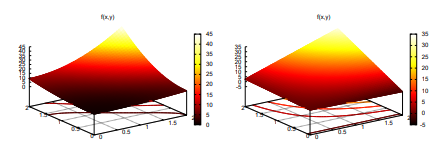
\includegraphics[width=0.7\linewidth]{img_33}
		\caption{Approximation of a 2D quadratic function (left) by a 2D bilinear
			function (right) using the Galerkin or least squares method.}
		\label{fig:img_33}
	\end{figure}
	
	\section[Implementation]{Implementation}
	\label{sec:sec_8_3}
	\noindent The least\textunderscore squares function from Section \hyperref[sec:sec_2_8]{2.8} and/or the file \href{https://github.com/hplgit/INF5620/blob/master/src/fem/fe_approx1D.py}{approx1D.py} can with very small modifications solve $2 \mathrm{D}$ approximation problems. First, let Omega now be a list of the intervals in $x$ and $y$ direction. For example, $\Omega=\left[0, L_{x}\right] \times\left[0, L_{y}\right]$ can be represented by Omega $=\left[\left[0, L_{-} \mathrm{x}\right],\left[0, \mathrm{~L}_{-} \mathrm{y}\right]\right]$. Second, the symbolic integration must be extended to $2 \mathrm{D}$ :
	\begin{lstlisting}[numbers=none]
		import sympy as sp
		
		integrand = psi[i]*psi[j]
		I = sp.integrate(integrand,
		
		(x, Omega[0][0], Omega[0][1]),
		(y, Omega[1][0], Omega[1][1]))	
	\end{lstlisting}
	provided integrand is an expression involving the sympy symbols x and y. The
	2D version of numerical integration becomes
	\begin{lstlisting}[numbers=none]
		if isinstance(I, sp.Integral):
		integrand = sp.lambdify([x,y], integrand)
		I = sp.mpmath.quad(integrand,
		[Omega[0][0], Omega[0][1]],
		[Omega[1][0], Omega[1][1]])	
	\end{lstlisting}
	The right-hand side integrals are modified in a similar way.
	
	Third, we must construct a list of $2 \mathrm{D}$ basis functions. Here are two examples based on tensor products of $1 \mathrm{D}$ "Taylor-style" polynomials $x^{i}$ and $1 \mathrm{D}$ sine functions $\sin ((i+1) \pi x)$ :
	\begin{lstlisting}[numbers=none]
		def taylor(x, y, Nx, Ny):
		return [x**i*y**j for i in range(Nx+1) for j in range(Ny+1)]
		
		def sines(x, y, Nx, Ny):
		return [sp.sin(sp.pi*(i+1)*x)*sp.sin(sp.pi*(j+1)*y)
		for i in range(Nx+1) for j in range(Ny+1)]	
	\end{lstlisting}
	The complete code appears in \href{http://tinyurl.com/jvzzcfn/fem/fe_approx2D.py}{approx2D.py.}
	
	The previous hand calculation where a quadratic f was approximated by a
	bilinear function can be computed symbolically by
	\begin{lstlisting}[numbers=none]
		>>> from approx2D import *
		>>> f = (1+x**2)*(1+2*y**2)
		>>> psi = taylor(x, y, 1, 1)
		>>> Omega = [[0, 2], [0, 2]]
		>>> u = least_squares(f, psi, Omega)
		>>> print u
		8*x*y - 2*x/3 + 4*y/3 - 1/9
		>>> print sp.expand(f)
		2*x**2*y**2 + x**2 + 2*y**2 + 1	
	\end{lstlisting}
	We may continue with adding higher powers to the basis:
	\begin{lstlisting}[numbers=none]
		>>> psi = taylor(x, y, 2, 2)
		>>> u = least_squares(f, psi, Omega)
		>>> print u
		2*x**2*y**2 + x**2 + 2*y**2 + 1
		>>> print u-f
		0	
	\end{lstlisting}
	For $N_{x} \geq 2$ and $N_{y} \geq 2$ we recover the exact function $f$, as expected, since in that case $f \in V$ (see Section \hyperref[sec:sec_2_5]{2.5}).
	\bigbreak 
	
	\section[Extension to 3D]{Extension to 3D}
	\label{sec:sec_8_4}
	\noindent Extension to 3D is in principle straightforward once the $2 \mathrm{D}$ extension is understood. The only major difference is that we need the repeated outer tensor product,
	$$
	V=V_{x} \otimes V_{y} \otimes V_{z}.
	$$
	In general, given vectors (first-order tensors) $a^{(q)}=\left(a_{0}^{(q)}, \ldots, a_{N_{q}}^{(q)}, q=0, \ldots, m\right.$, the tensor product $p=a^{(0)} \otimes \cdots \otimes a^{m}$ has elements
	$$
	p_{i_{0}, i_{1}, \ldots, i_{m}}=a_{i_{1}}^{(0)} a_{i_{1}}^{(1)} \cdots a_{i_{m}}^{(m)} .
	$$
	The basis functions in $3 \mathrm{D}$ are then
	$$
	\psi_{p, q, r}(x, y, z)=\hat{\psi}_{p}(x) \hat{\psi}_{q}(y) \hat{\psi}_{r}(z),
	$$
	with $p \in \mathcal{I}_{x}, q \in \mathcal{I}_{y}, r \in \mathcal{I}_{z}$. The expansion of $u$ becomes
	$$
	u(x, y, z)=\sum_{p \in \mathcal{I}_{x}} \sum_{q \in \mathcal{I}_{y}} \sum_{r \in \mathcal{I}_{z}} c_{p, q, r} \psi_{p, q, r}(x, y, z) .
	$$
	A single index can be introduced also here, e.g., $i=N_{x} N_{y} r+q_{N} x+p, u=$ $\sum_{i} c_{i} \psi_{i}(x, y, z)$.
	\begin{mybox}
		\textbf{Use of tensor product spaces.}
		
		\noindent Constructing a multi-dimensional space and basis from tensor products of 1D spaces is a standard technique when working with global basis functions. In the world of finite elements, constructing basis functions by tensor products is much used on quadrilateral and hexahedra cell shapes, but not on triangles and tetrahedra. Also, the global finite element basis functions are almost exclusively denoted by a single index and not by the natural tuple of indices that arises from tensor products.
	\end{mybox}
\clearpage
\end{document} 
